\addcontentsline{toc}{section}{Introduction}
\section*{Introduction}
Ce chapitre est consacré à la modélisation et à l’implémentation de notre model d’IA et du backend Django.  Le model permettre d’offrir deux Rest API (un pour l’authentification et le second pour l’identification). Ainsi n’importe quel client web, mobile ou desktop pourra consommer les Apis.  La modélisation fera l’analyse du contexte qui nous permet de sortir les différentes fonctionnalités que nous allons mettre en exergue à travers un diagramme de cas d’utilisation. Dans l’implémentation, nous abordons les détails relatifs à l’installation des outils de développement et de test, une esquisse du système, Enfin, nous présentons certaines parties du code source.   
%\paragraph{}Ce chapitre est consacré à 
%l  
\section{architecture du système}
\paragraph{}Le TDNN (Time Delay Neural Network) est un type de réseau de neurones récurrent utilisé pour la reconnaissance de la parole et la modélisation de la langue. Il est souvent utilisé dans les systèmes de reconnaissance automatique de la parole, tels que les systèmes de reconnaissance de locuteurs.
\paragraph{}Les x-vectors sont des vecteurs de caractéristiques extraits de l'entrée audio, qui sont utilisés pour la reconnaissance de locuteurs. Les TDNN sont souvent utilisés pour extraire les x-vectors à partir de l'audio.
\paragraph{}L'architecture d'un TDNN utilisé pour extraire les x-vectors est constituée de plusieurs couches de neurones, chacune avec une taille de fenêtre différente. Chaque couche est composée de plusieurs neurones qui sont connectés à des entrées audio avec un retard temporel.
\paragraph{}Le retard temporel est utilisé pour permettre au réseau de traiter des informations audio qui se produisent à différents moments dans le temps. Par exemple, une couche peut être configurée pour traiter des informations audio qui ont été enregistrées 100 millisecondes avant l'instant actuel, tandis qu'une autre couche peut traiter des informations audio enregistrées 200 millisecondes avant l'instant actuel voir figure \ref{fig:2-clab-3}.
\paragraph{}Les sorties de chaque couche sont ensuite combinées pour produire un vecteur de caractéristiques global, qui est utilisé comme x-vector pour la reconnaissance de locuteurs.
\paragraph{}En résumé, l'architecture d'un TDNN utilisé pour extraire les x-vectors est généralement constituée de plusieurs couches de neurones, chacune avec une taille de fenêtre différente et connectée à des entrées audio avec un retard temporel. Les sorties de chaque couche sont combinées pour produire un vecteur de caractéristiques global, qui est utilisé comme x-vector pour la reconnaissance de locuteurs.

\section{Le model}
\paragraph{}Tel que nous l’avons énoncé dans les parties précédentes, De nombreux modèles neuronaux peuvent être utilisés pour aborder ce type de tâche. Dans cette étude, nous nous concentrerons sur un classificateur TDNN (xvector).
\paragraph{}Comme le montre la figure ci-dessous, l’architecture TDNN est basée sur la topologie à vecteur x (xvector), et introduit plusieurs améliorations pour les IA dans le domaine du traitement des signaux vocaux.
\paragraph{}La couche de pooling utilise un mécanisme d'attention dépendant du canal et du contexte, ce qui permet au réseau d'attirer l'attention sur différents frames par canal. Des blocs SqueezeExcitation unidimensionnels (SE) redimensionnent les canaux des cartes de caractéristiques de niveau de frame intermédiaires pour insérer des informations de contexte global dans les blocs de convolution qui fonctionnent localement. Ensuite, l'intégration de blocs Res2 unidimensionnels améliore les performances tout en réduisant simultanément le nombre total de paramètres en utilisant des convolutions groupées de manière hiérarchique.
\paragraph{}Enfin, l'agrégation de fonctionnalités multi-couches (MFA) fusionne des informations complémentaires avant le pooling de statistiques en concaténant la carte de caractéristiques de niveau de frame finale avec des cartes de caractéristiques intermédiaires de couches précédentes.
\paragraph{}Le réseau est entraîné en optimisant la perte AAMsoftmax sur les identités de locuteurs dans le corpus d'entraînement. L'AAM-softmax est une amélioration puissante par rapport à la perte softmax régulière dans le contexte des problèmes de classification et de vérification fine. Il optimise directement la distance cosinus entre les embeddings de locuteur.


\begin{figure}[h]
    \centering
    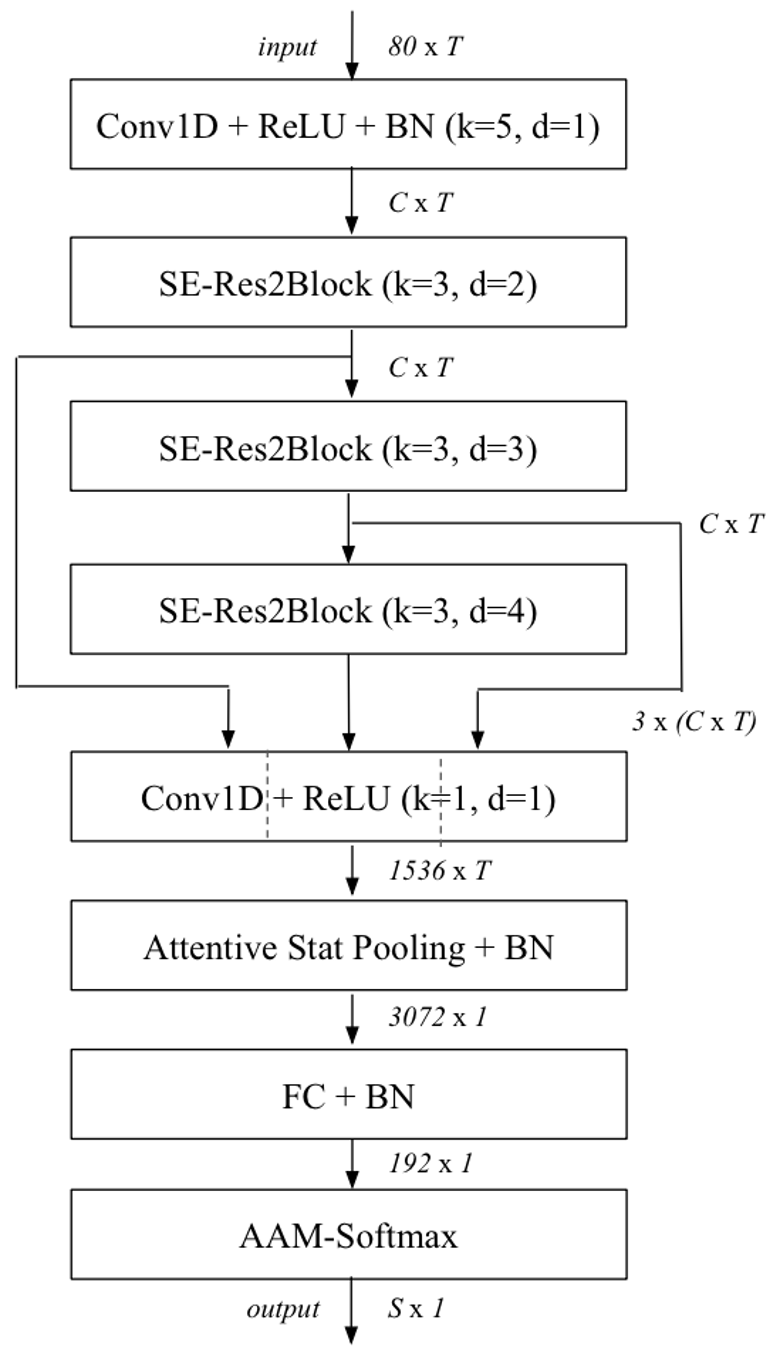
\includegraphics[width=0.5\textwidth]{3chap1}
    \caption{Structure d'un RN de type TDNN}
    \label{fig:3chap1}
\end{figure}
\paragraph{}


\section{Les données d'entrainement}
L’entrainement se fera avec un petit ensemble de données open source appelé minilibrispeech à laquelle nous avons ajouté des données vocales d’un certain nombre de personnalités politiques et médias. Tous les fichiers vocaux sonnt au format .flac, channel Mono et de frequence 16 KHz.

\begin{figure}[h]
    \centering
    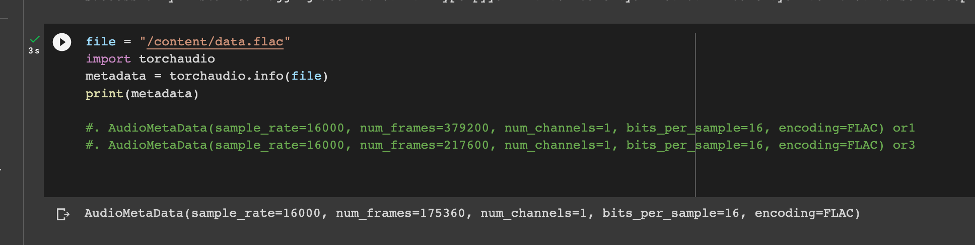
\includegraphics[width=1\textwidth]{3chap2}
    \caption{caractéristiques des enregistrements vocaux}
    \label{fig:3chap2}
\end{figure}
\paragraph{}Nous avons ainsi, un dataset d’une trentaine d’empreinte vocale, qui ne contient que quelques heures de données de formation. Nous avons aussi mis en place un data pipeline qui à partir d’un API Rest peux servir à étendre le dataset. 


\begin{figure}[h]
    \centering
    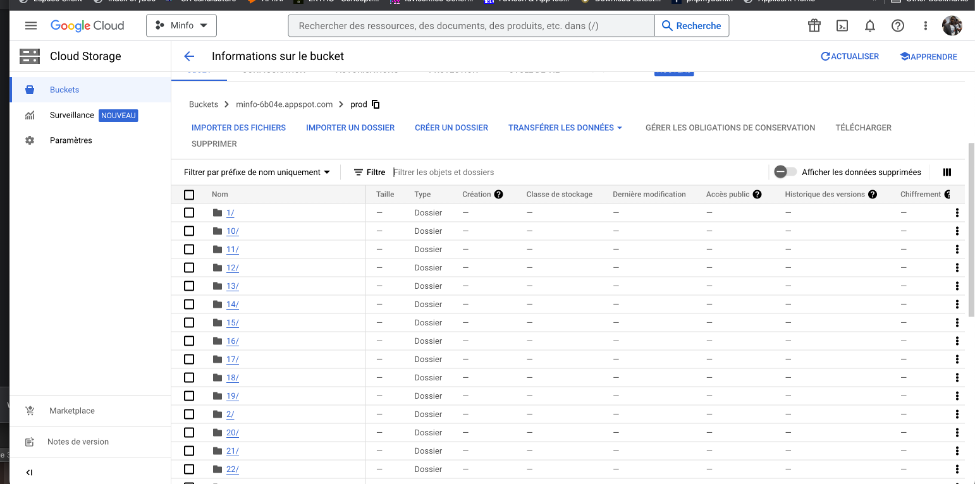
\includegraphics[width=1\textwidth]{3chap3}
    \caption{Le dataset dansle bucket Cloud Storage}
    \label{fig:3chap3}
\end{figure}


\begin{figure}[h]
    \centering
    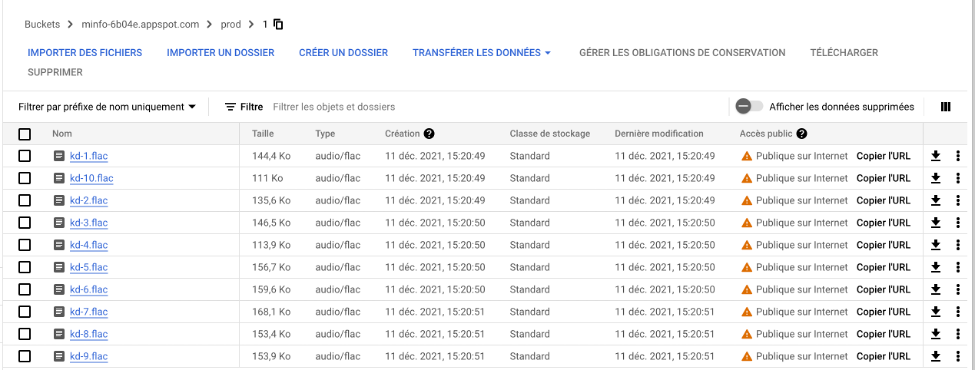
\includegraphics[width=1\textwidth]{3chap4}
    \caption{enregistrementsvocaux d'un seul utilisateur}
    \label{fig:3chap4}
\end{figure}

\section{Le code}
Pour l’entrainement, on va cloner le répertoire  \href{ https://github.com/kadersaka/minfo_speaker_identification}{github.com/kadersaka/minfo-speaker-identification}. On y trouve un ensemble de fichiers et de dossiers, dont :

\begin{itemize}
    \item \textbf{train.py }: le fichier de code principal, décrit l'ensemble du processus d’entrainement.
    \item \textbf{train.yaml }: le fichier d'hyperparamètres, définit tous les paramètres d'exécution.
	\item \textbf{custom-model.py } : un fichier contenant la définition d'un module PyTorch dont on aura besoin pour l’inférence.
	\item \textbf{mini-librispeech-prepare.py} : si nécessaire, télécharge et prépare les manifestes de données si elles ne sont pas encore dans l’environnement d’entrainement.
\end{itemize}
Pour entrainer le modèle speaker-id, on va exécuter la commande :

\section{Installations}
La première chose à faire est de créer un notebook Colab.  Ensuite, nous allons activer l’exécution en mode GPU car nous en auront besoin pour l’entrainement. Puis il faudra cloner le code du répertoire GitHub ci-dessus; (voir figure \ref{fig:3chap5}).
\begin{figure}[h]
    \centering
    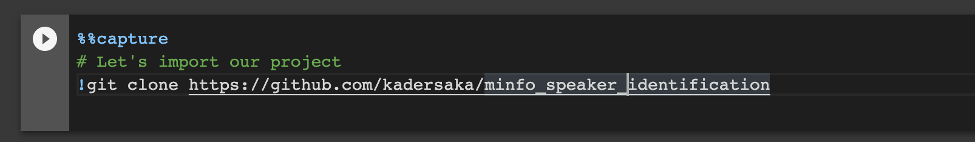
\includegraphics[width=1\textwidth]{3chap5}
    \caption{enregistrementsvocaux d'un seul utilisateur}
    \label{fig:3chap5}
\end{figure}
Ensuite il faudra installer la librairie SpeechBrain (voir figure \ref{fig:3chap6}).
\begin{figure}[h]
    \centering
    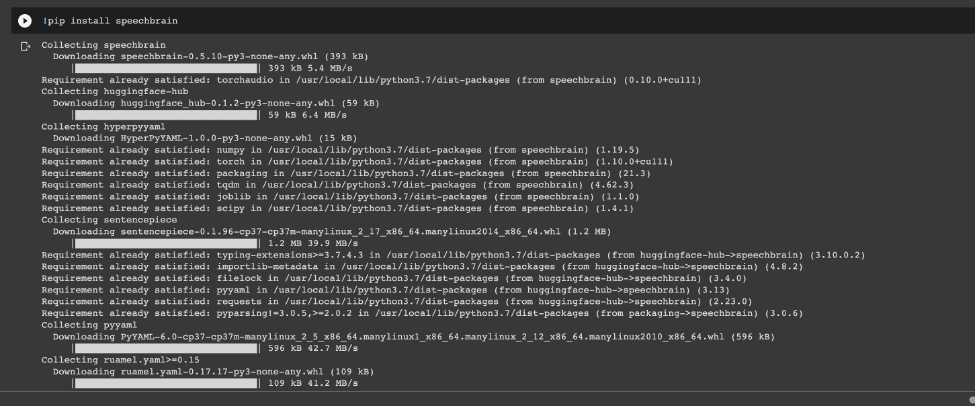
\includegraphics[width=1\textwidth]{3chap6}
    \caption{enregistrementsvocaux d'un seul utilisateur}
    \label{fig:3chap6}
\end{figure}

\section{Preparation des données}
A cette étape la première chose à faire est de donner les autorisations au fichier Colab de pouvoir accéder au Bucket du Cloud Storage pour récupérer le dataset. Ensuite, nous utilisons GsUtils pour la gestion des données du Bucket, notamment leur copie de cloud Storage vers l’environnement local du Colab (voir figure \ref{fig:3chap7}).

\begin{figure}[h]
    \centering
    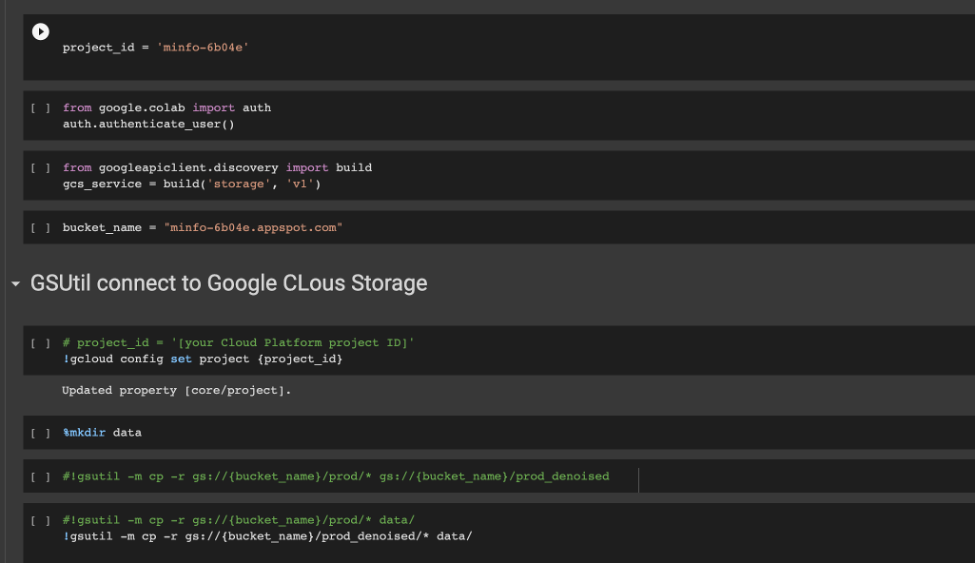
\includegraphics[width=1\textwidth]{3chap7}
    \caption{récupération des données}
    \label{fig:3chap7}
\end{figure}
Après avoir récupéré le dataset, nous pouvons maintenant préparer les données.  L'objectif de la préparation des données est de créer les fichiers manifestes de données. Ces fichiers indiquent à SpeechBrain où trouver les données audio et leur classification au niveau de l'énoncé correspondante. Ce sont des fichiers texte écrits dans les formats populaires CSV et JSON  (voir figure \ref{fig:3chap8}).
\begin{figure}[h]
    \centering
    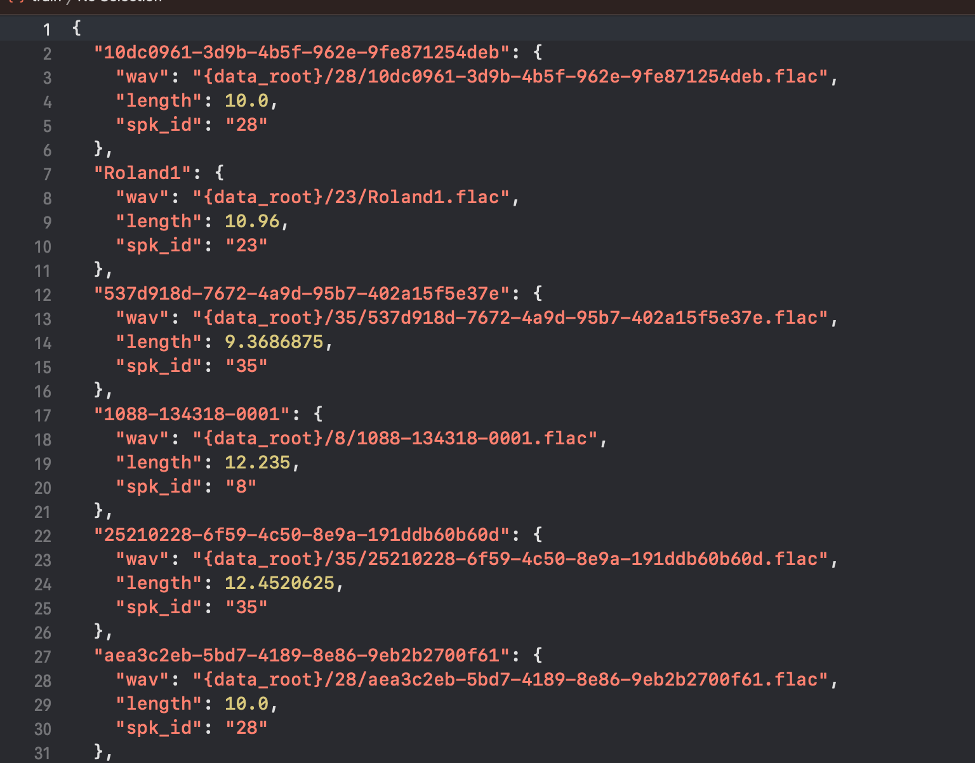
\includegraphics[width=1\textwidth]{3chap8}
    \caption{Fichier manifestes d'entrainement}
    \label{fig:3chap8}
\end{figure}

Comme vous pouvez le voir, nous avons une structure hiérarchique spécifiant tous les champs nécessaires à la tâche adressée. Par exemple, nous rapportons le chemin de l'enregistrement vocal, sa durée en secondes (nécessaire si nous voulons trier les phrases avant de créer les mini-lots) et l'identité (ID) du locuteur dans l'enregistrement donné.
Il faut préciser qu’a cette étape le dataset est divise en trois partitions, chacun avec son fichier manifest :
\begin{itemize}
    \item le premier pour les l’entrainement
    \item le second pour les test
    \item et le troisième pour la validation du model
\end{itemize}

\section{Entrainement du modèle TDNN}

Nous allons former le modèle basé sur TDNN utilisé pour les X-Vector. La mise en commun statistique est utilisée au-dessus des couches convolutives (CNN) pour convertir un vocal de longueur variable en incorporations de longueur fixe. Les parametres sont sur le fichier train.yaml

\begin{figure}[h]
    \centering
    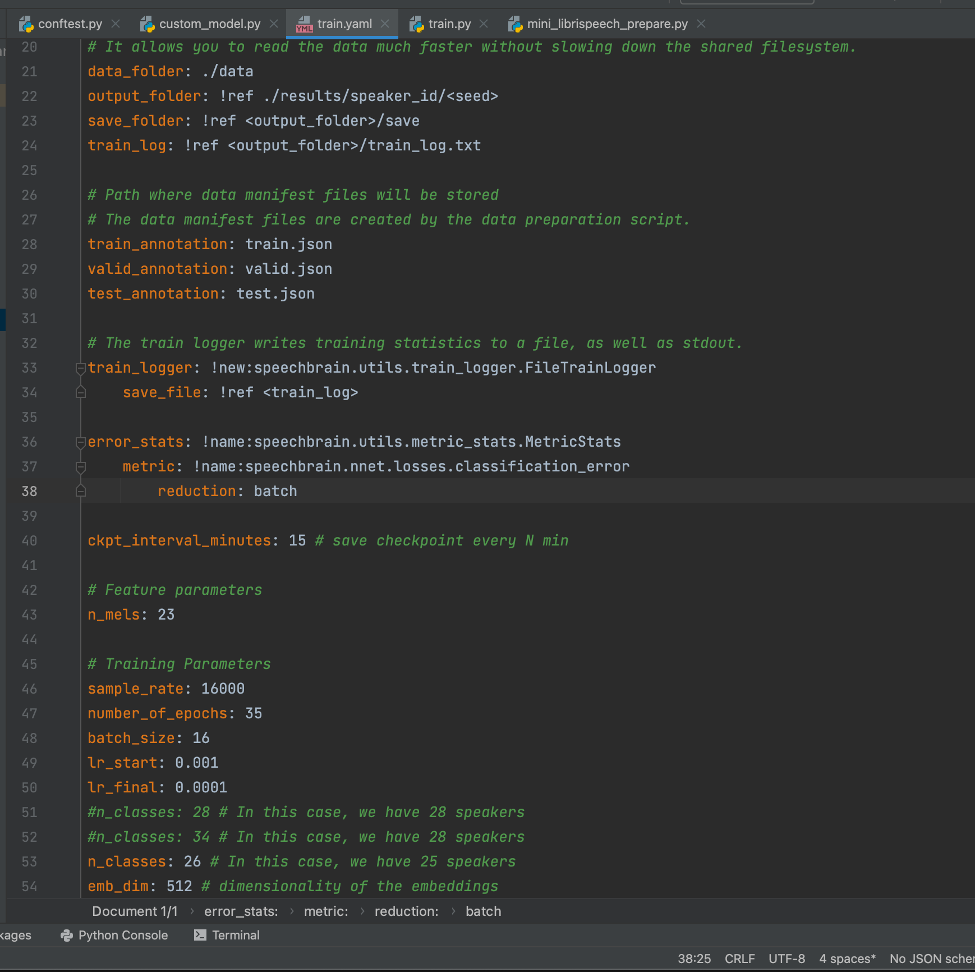
\includegraphics[width=1\textwidth]{3chap9}
    \caption{Fichier des paramètres d'entrainement}
    \label{fig:3chap9}
\end{figure}
Dans ce fichier  (voir figure \ref{fig:3chap9}):
\begin{itemize}
    \item Dans la première partie, nous spécifions quelques paramètres de base, tels que le seed, le chemin du dossier qui contiendra nos fichiers vocaux et le chemin du dossier de sortie (voir figure \ref{fig:3chap10}):
    \begin{figure}[h]
		\centering
		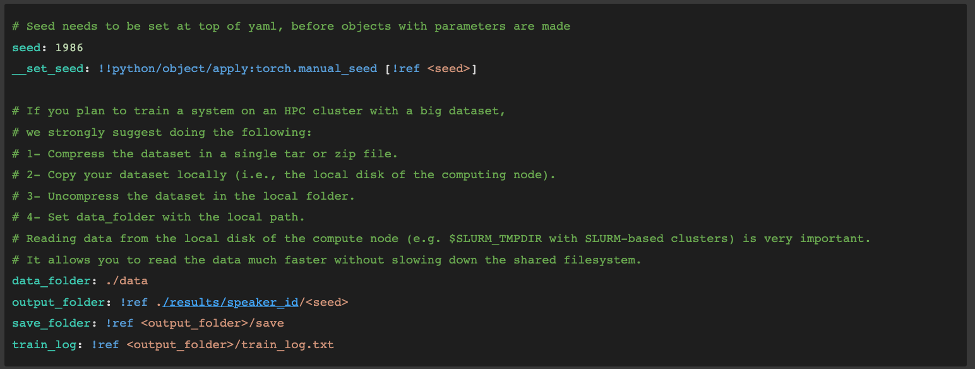
\includegraphics[width=1\textwidth]{3chap10}
		\caption{paramètres de base d'entrainement}
		\label{fig:3chap10}
	\end{figure}
    \item Nous spécifions ensuite le chemin des fichiers manifestes de données pour l’entrainement, la validation et le test voir figure \ref{fig:3chap11}):
	\begin{figure}[h]
		\centering
		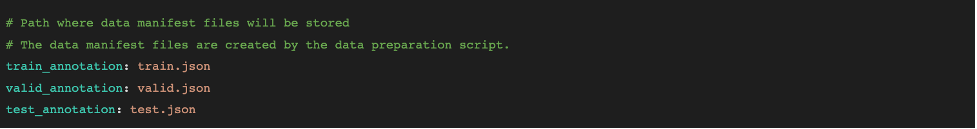
\includegraphics[width=1\textwidth]{3chap11}
		\caption{paramètres des chemins des fichiers manifestes}
		\label{fig:3chap11}
	\end{figure}
	\\Ces fichiers seront créés automatiquement lors de l'appel du script de préparation des données (mini\_librispeech\_prepare.py) à partir du fichier d’entrainement (train.py).
	\item Ensuite, nous configurons le train\_logger et déclarons les objets error\textunderscore stats qui recueilleront des statistiques sur le taux d'erreur de classification (voir figure \ref{fig:3chap12}):
	\begin{figure}[h]
		\centering
		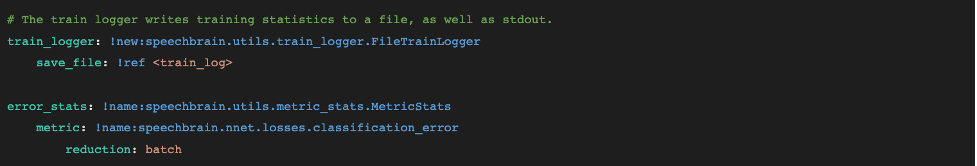
\includegraphics[width=1\textwidth]{3chap12}
		\caption{paramètres des chemins des fichiers manifestes}
		\label{fig:3chap12}
	\end{figure}
	
	\item Nous pouvons maintenant spécifier certains hyperparamètres d'entraînement tels que le nombre d'époques, la taille du lot, le taux d'apprentissage, le nombre d'époques et la dimensionnalité d'intégration (voir figure \ref{fig:3chap13}).
	\begin{figure}[h]
		\centering
		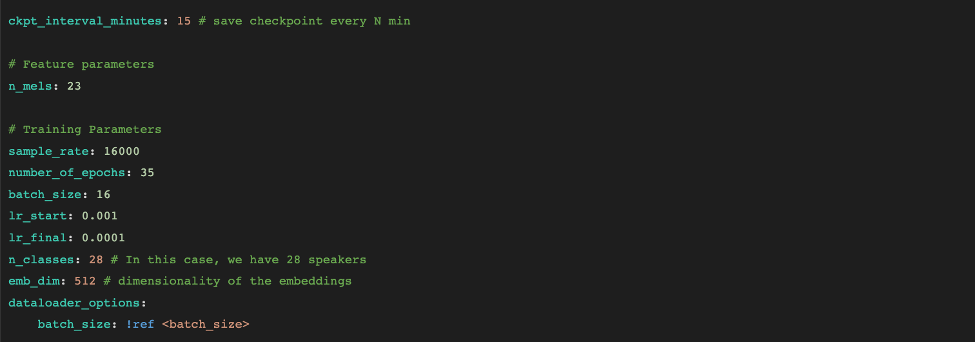
\includegraphics[width=1\textwidth]{3chap13}
		\caption{Autres paramètres}
		\label{fig:3chap13}
	\end{figure}

\end{itemize}

La variable ckpt\_interval\_minutes peut être utilisée pour enregistrer des points de contrôle toutes les N minutes au cours d'une période d'entraînement. Dans certains cas, une époque peut prendre plusieurs heures, et enregistrer périodiquement le point de contrôle est une bonne pratique sûre.  
Nous pouvons maintenant définir les modules les plus importants qui sont nécessaires pour former notre modèle (voir figure \ref{fig:3chap14})

\begin{figure}[h]
	\centering
	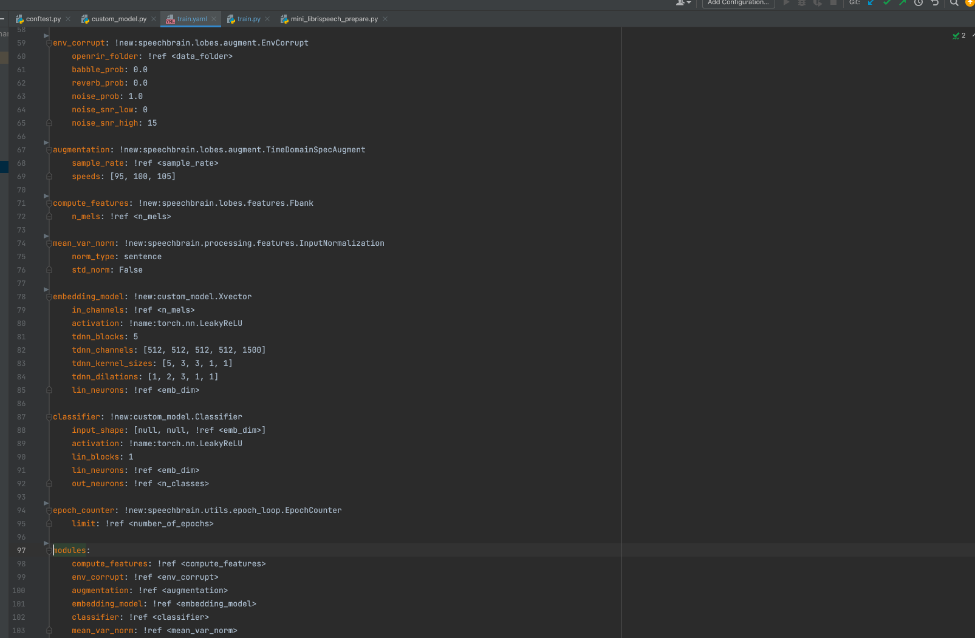
\includegraphics[width=1\textwidth]{3chap14}
	\caption{Paramètres d'augmentation des données avec les bruits}
	\label{fig:3chap14}
\end{figure}

La partie d'augmentation est basée à la fois sur env\_corrupt (qui ajoute du bruit et de la réverbération) et augmentation (qui ajoute des pertes de temps/fréquence et un changement de vitesse). 
Nous terminons la spécification des hyperparamètres avec la déclaration de l'optimiseur, de l'ordonnanceur du taux d'apprentissage et du pointeur de contrôle :
\begin{figure}[h]
	\centering
	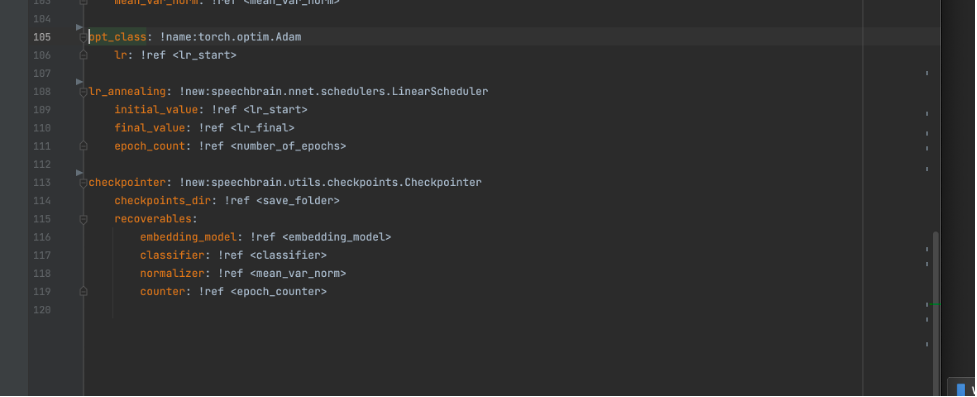
\includegraphics[width=1\textwidth]{3chap15}
	\caption{Paramètres d'augmentation des données avec les bruits}
	\label{fig:3chap15}
\end{figure}

Dans notre  cas, nous utilisons Adam comme optimiseur et une décroissance linéaire du taux d'apprentissage sur les 15 époques.
Adam (Adaptive Moment Estimation) est un optimiseur très populaire pour l'apprentissage profond, car il combine les avantages de deux autres optimiseurs, à savoir la descente de gradient stochastique (SGD) avec moment et la méthode d'estimation adaptative de la moyenne du carré des gradients (RMSProp). L'optimiseur Adam est très efficace pour résoudre des problèmes de gradient évanescents ou explosifs, car il utilise des moments d'ordre supérieur pour adapter le taux d'apprentissage pour chaque paramètre.
En pratique, l'utilisation de la décroissance linéaire du taux d'apprentissage avec l'optimiseur Adam peut améliorer la stabilité et la convergence du modèle, en particulier pour les problèmes de grande envergure avec des données complexes. Cependant, il est important de noter que le taux d'apprentissage doit être choisi avec soin, car une décroissance trop rapide peut conduire à une convergence lente ou à des minima locaux, tandis qu'une décroissance trop lente peut entraîner une instabilité ou une divergence.
Voici donc comment les objets, les fonctions et les hyperparamètres déclarés dans le fichier yaml sont utilisés dans train.py pour implémenter le classifieur.
Parcourrons maintenant le fichier principal train.py (voir figure \ref{fig:3chap16}):

\begin{figure}[h]
	\centering
	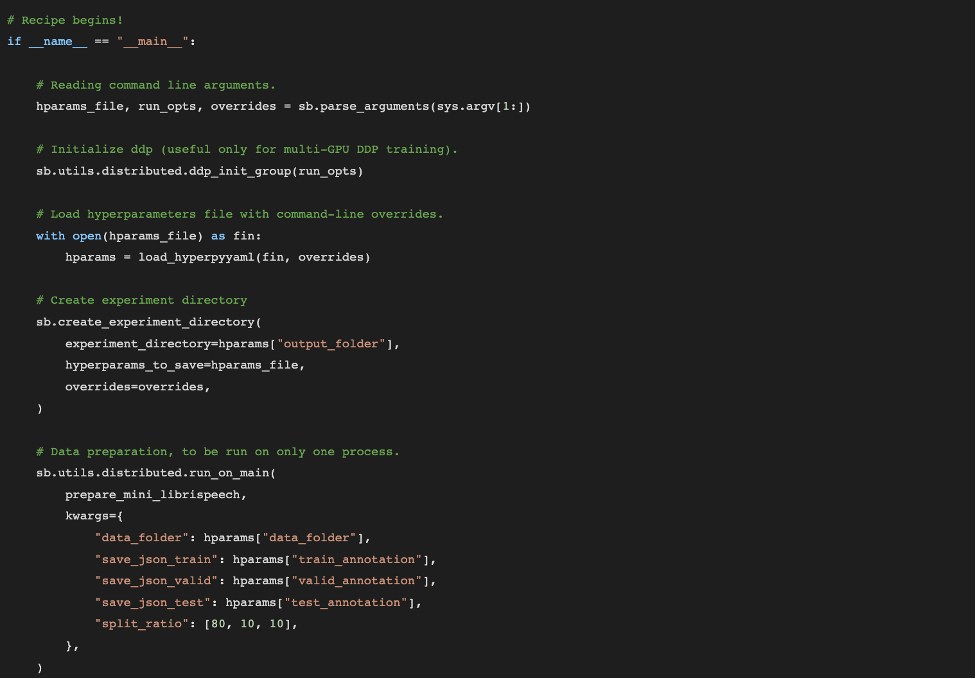
\includegraphics[width=1\textwidth]{3chap16}
	\caption{Code d'entrainement}
	\label{fig:3chap16}
\end{figure}


Nous effectuons ici quelques opérations préliminaires telles que l'analyse de la ligne de commande, l'initialisation des données distribuées en parallèle (nécessaire si plusieurs GPU sont utilisés), la création du dossier de sortie et la lecture du fichier yaml afin de récupérer les paramètres par défaut.
Après lecture du fichier yaml avec load\_hyperpyyaml, tous les objets déclarés dans les fichiers d'hyperparamètres sont initialisés et disponibles sous forme de dictionnaire (ainsi que les autres fonctions et paramètres rapportés dans le fichier yaml). Par exemple, nous aurons hparams['embedding\_model'], hparams['classifier'], hparams['batch\_size'], etc.
Nous exécutons également le script de préparation des données prepare\_mini\_librispeech qui crée les fichiers manifestes de données(distribuées à 80\% pour l'entrainement, 10\% pour la validation, et 10\% pour les tests). Il est encapsulé avec sb.utils.distributed.run\_on\_main car cette opération écrit les fichiers manifestes sur le disque.
\\Nous appelons ensuite la fonction qui crée les objets de l'ensemble de données pour la formation, la validation et le test.

\begin{figure}[h]
	\centering
	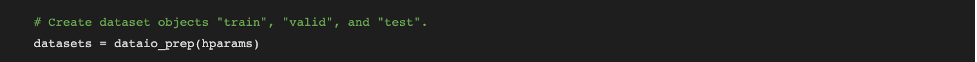
\includegraphics[width=1\textwidth]{3chap17}
	\caption{commande de separation des données}
	\label{fig:3chap17}
\end{figure}

\begin{figure}[h]
	\centering
	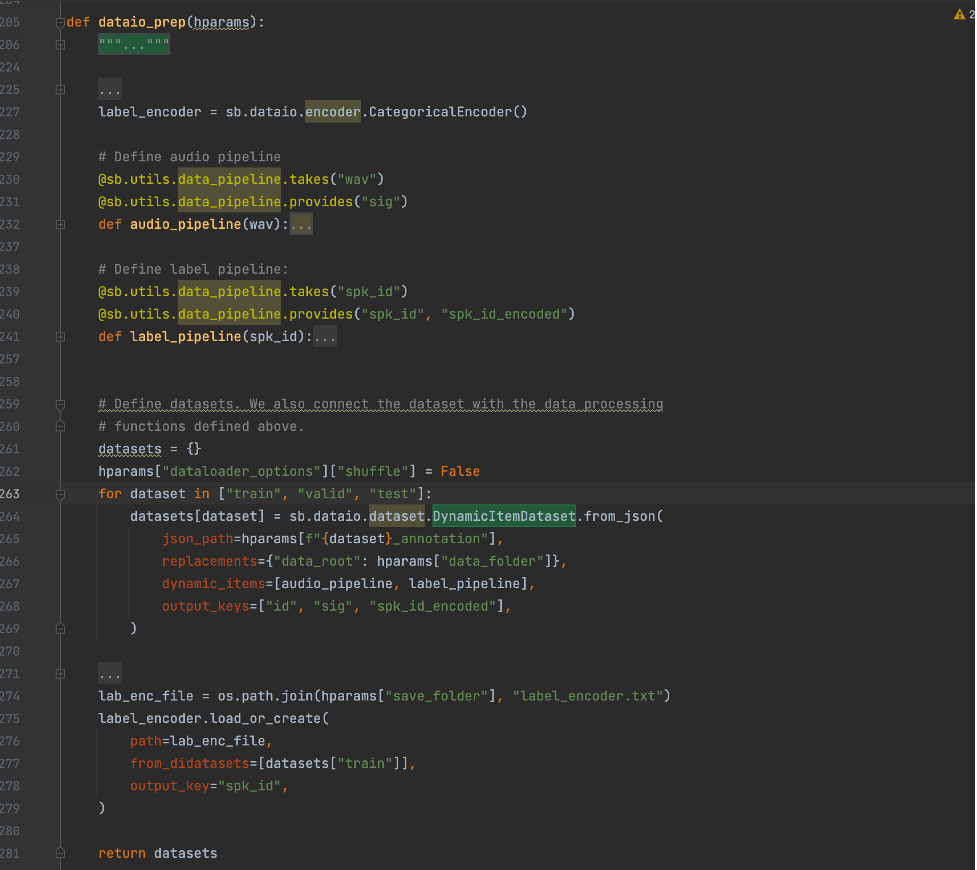
\includegraphics[width=1\textwidth]{3chap18}
	\caption{Code de separation des données}
	\label{fig:3chap18}
\end{figure}

La première partie est juste une déclaration de CategoricalEncoder qui sera utilisée pour convertir les étiquettes catégorielles en leurs index correspondants.
Nous exposons ensuite  les fonctions de traitement audio et label.
La fonction  audio\_pipeline prend le chemin d’un signal audio (wav) et le lit. Il renvoie un objet tensor contenant la phrase vocale lue. L'entrée en paramètre de cette fonction (c'est-à-dire le fichier wav) doit avoir le même nom que la clé correspondante dans le fichier manifeste de données généré:
Ex : 
\begin{figure}[h]
	\centering
	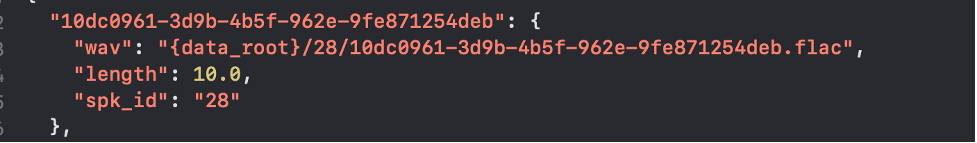
\includegraphics[width=1\textwidth]{3chap19}
	\caption{ligne du fichier manifeste}
	\label{fig:3chap19}
\end{figure}

De même, nous définissons une autre fonction appelée label\_pipeline pour traiter les étiquettes au niveau de l'énoncé et les mettre dans un format utilisable par le modèle défini. La fonction lit la chaîne spk\_id définie dans le fichier JSON et l'encode avec l'encodeur catégoriel.
Nous créons ensuite un objet de type DynamicItemDataset et le connectons aux fonctions de traitement définies ci-dessus. Nous définissons les clés de sortie souhaitées à exposer. Ces clés seront disponibles dans la classe brain dans la variable batch comme :
\begin{itemize}
    \item batch.id
    \item lot.sig
    \item lot.spk\_id\_encoded
\end{itemize}

La dernière partie de la fonction est dédiée à l'initialisation de l'encodeur d'étiquettes. L'encodeur d'étiquettes prend en entrée le jeu de données d'apprentissage et attribue un index différent à toutes les entrées spk\_id trouvées. Ces index correspondront aux index de sortie du classifieur.
Après la définition des jeux de données, la fonction main peut procéder à l'initialisation et à l'utilisation de la classe brain :

\begin{figure}[h]
	\centering
	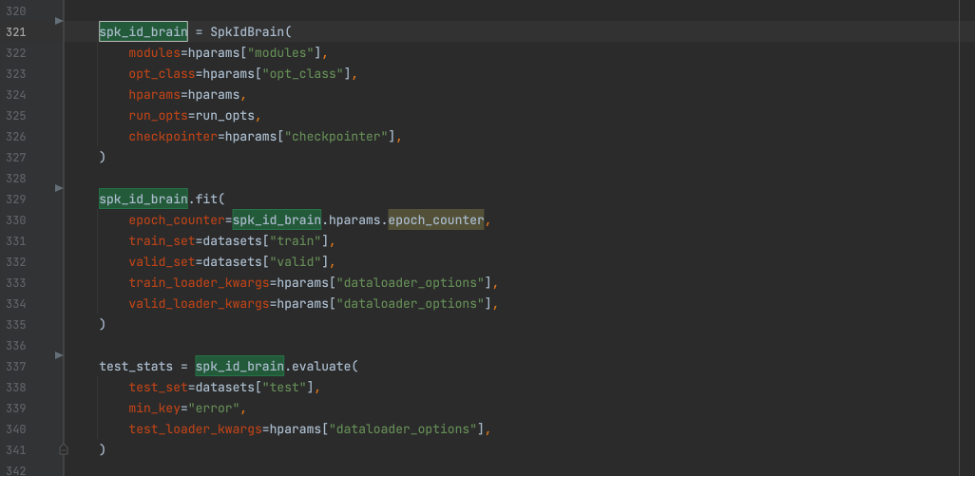
\includegraphics[width=1\textwidth]{3chap20}
	\caption{Classe Brain}
	\label{fig:3chap20}
\end{figure}

La méthode d'ajustement effectue l’entrainement, tandis que le test est effectué avec celui d'évaluation. Les chargeurs de données d'entraînement et de validation sont fournis en entrée de la méthode d'ajustement, tandis que l'ensemble de données de test est introduit dans la méthode d'évaluation.
Examinons maintenant les méthodes les plus importantes définies dans la classe brain:

\subsection*{Les Calculateurs}
Commençons par la fonction forward, qui définit tous les calculs nécessaires pour transformer l'audio d'entrée en prédictions de sortie.

\begin{figure}[h]
	\centering
	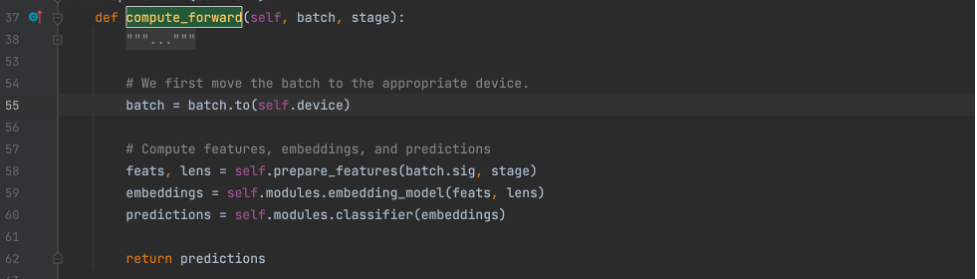
\includegraphics[width=1\textwidth]{3chap21}
	\caption{compute forward}
	\label{fig:3chap21}
\end{figure}

Dans ce cas, la chaîne de calcul est très simple. Nous plaçons simplement le lot sur le bon appareil et calculons les caractéristiques acoustiques. Nous traitons ensuite les caractéristiques avec l'encodeur TDNN qui produit un objet tensor de taille fixe (notre. X-Vector). Ce dernier alimente un classifieur qui sort les probabilités a posteriori sur les N classes (ici les 31 locuteurs). L'augmentation des données est ajoutée dans la méthode prepare\_features :

\begin{figure}[h]
	\centering
	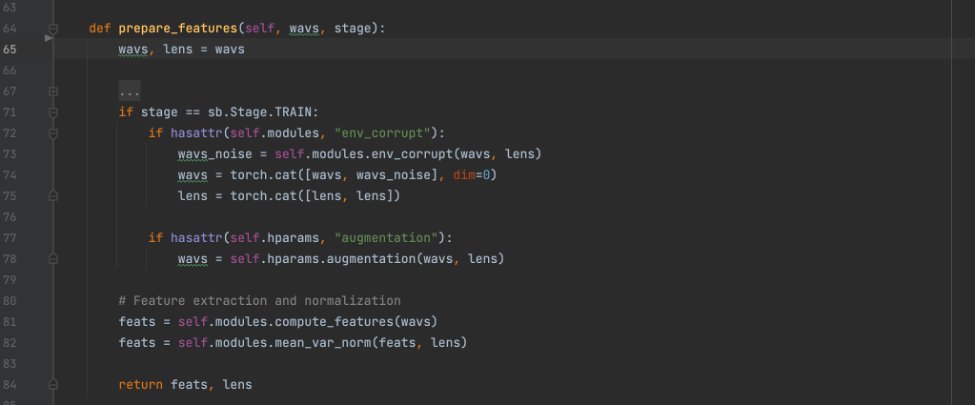
\includegraphics[width=1\textwidth]{3chap22}
	\caption{augmentation des données }
	\label{fig:3chap22}
\end{figure}

En particulier, lorsque la corruption (Fichiers parasites sonores) de l'environnement est déclarée dans le fichier yaml, nous concaténons dans le même lot la version propre et la version augmentée des signaux parasites.
Cette approche double la taille du lot, mais elle implémente un régularisateur très puissant. Le fait d'avoir à la fois la version propre et la version bruyante du signal dans le même lot force le gradient à pointer dans une direction de l'espace des paramètres qui est robuste contre les distorsions du signal.

\subsection*{Objectifs de calcul}
Intéressons-nous maintenant à la méthode compute\_objectives qui prend en entrée les cibles, les prédictions, et estime une fonction de perte :

\begin{figure}[h]
	\centering
	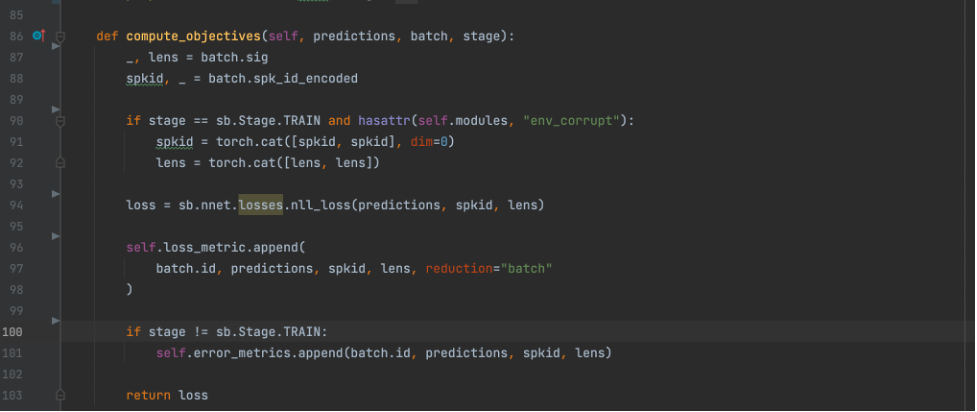
\includegraphics[width=1\textwidth]{3chap23}
	\caption{definition de la fonction de perte}
	\label{fig:3chap23}
\end{figure}
Les prédictions en entrée sont celles calculées dans la méthode directe. La fonction de coût est évaluée en comparant ces prédictions avec les étiquettes cibles. 

\subsection*{Les autres méthodes}
Au-delà de ces deux fonctions importantes, nous avons d'autres méthodes qui sont utilisées par l’IA. Le on\_state\_starts est appelé au début de chaque époque et il est utilisé pour configurer les trackers de statistiques. Le on\_stage\_end est appelé à la fin de chaque étape (par exemple, à la fin de chaque période d'entraînement) et s'occupe principalement de la gestion des statistiques, du recuit du taux d'apprentissage et des points de contrôle. 
\\Pour démarrer l’entraînement nous allons exécuter le code suivant :  
\textbf{python train.py train.yaml --number\_of\_epochs=15}

nous pouvons y passer des paramètres qui vont overrider les paramètres par défaut énoncés sur le fichier train.yaml
On observe sur la console que les pertes de validation et d’entrainement (loss function) diminuent très rapidement dans les premières époques. Ensuite, nous voyons essentiellement quelques améliorations mineures et des oscillations de performances.
\begin{figure}[h]
	\centering
	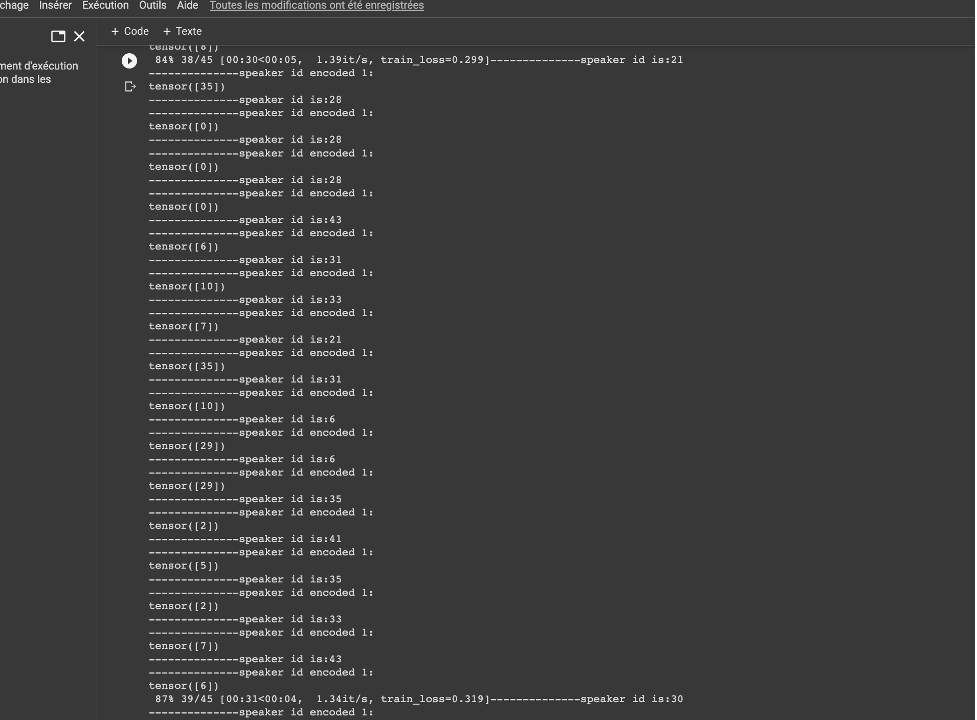
\includegraphics[width=1\textwidth]{3chap24}
	\caption{Logs de l’entrainement variation de la function loss}
	\label{fig:3chap24}
\end{figure}

\begin{figure}[h]
	\centering
	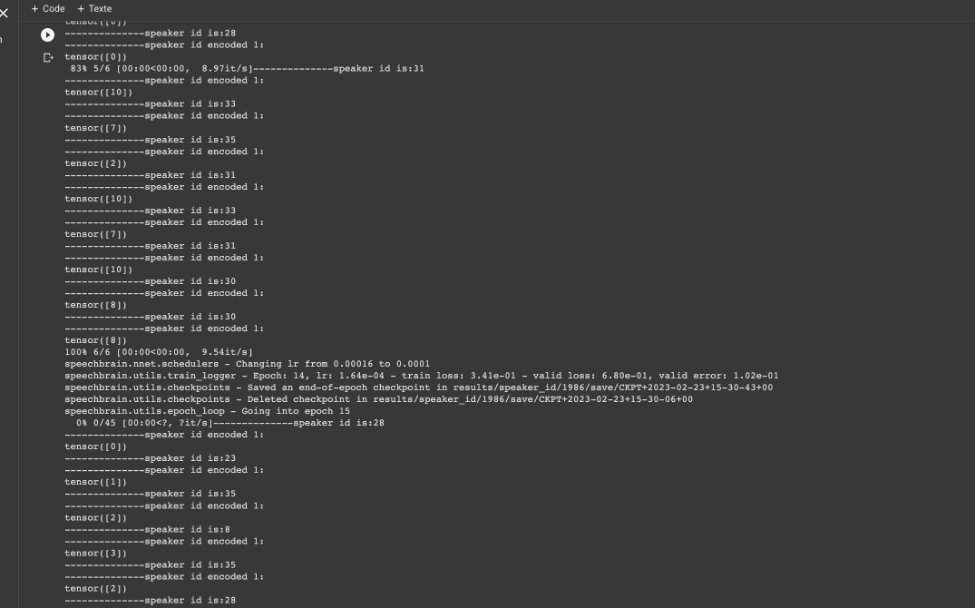
\includegraphics[width=1\textwidth]{3chap25}
	\caption{Logs de l’entrainement, passage de l’Epoch 14 à l’Epoch 15}
	\label{fig:3chap25}
\end{figure}

Voyons quels fichiers/dossiers sont générés dans le output\_folder spécifié :
\begin{itemize}
    \item \textbf{train\_log.txt} : contient les statistiques (par exemple, train\_loss, valid\_loss) calculées à chaque époque.
    \item \textbf{log.txt} : est un enregistreur plus détaillé contenant les horodatages pour chaque opération de base.
    \item \textbf{env.log} : affiche toutes les dépendances utilisées avec leur version correspondante (utile pour la réplicabilité).
    \item \textbf{train.py, hyperparams.yaml }: sont une copie du fichier d'expérience avec les hyperparamètres correspondants 
    \item \textbf{save} : est l'endroit où nous stockons le modèle généré.

\end{itemize}

Dans le dossier de sauvegarde, on a des sous-dossiers contenant les points de contrôle enregistrés lors de l'entraînement (au format CKPT+données+heure). Typiquement, on y trouve ici deux points de contrôle : le meilleur (c'est-à-dire le plus ancien) et dernier (c'est-à-dire le plus récent). 
\begin{figure}[h]
	\centering
	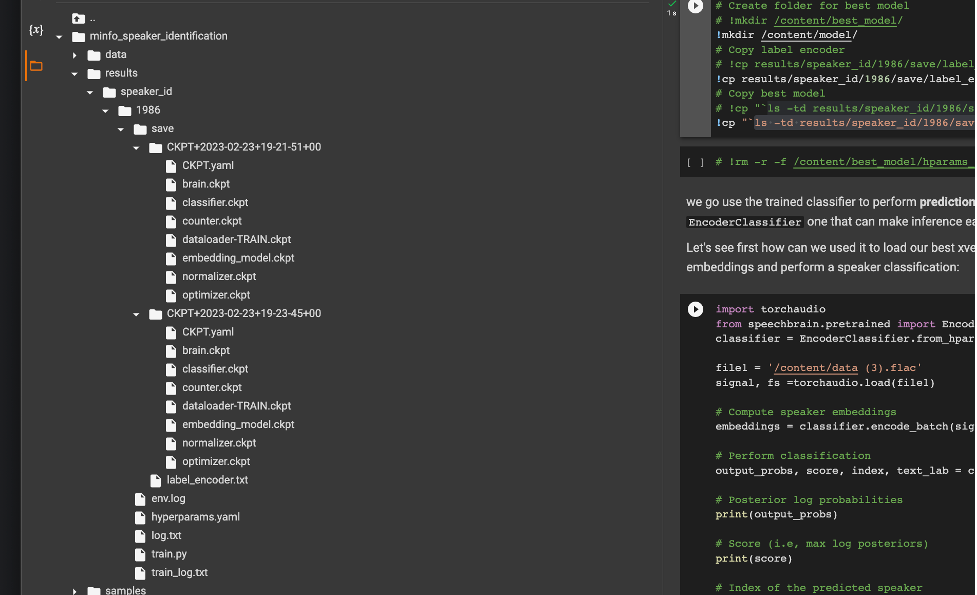
\includegraphics[width=1\textwidth]{3chap26}
	\caption{Les deux models }
	\label{fig:3chap26}
\end{figure}

À l'intérieur de chaque point de contrôle, nous stockons toutes les informations nécessaires pour reprendre l’entrainement (par exemple, les modèles, les optimiseurs, les planificateurs, le compteur d'époques, etc.). Les paramètres des modèles d'intégration sont rapportés dans le fichier embedding\_model.ckpt, tandis que ceux du classifieur sont dans classifier.ckpt. C'est juste un format binaire lisible avec torch.load.
Le dossier de sauvegarde contient également l'encodeur d'étiquette (label\_encoder.txt), qui mappe chaque entrée d'id de locuteur à leurs index correspondants.
A la fin de l’entrainement, l'erreur de validation doit passer à zéro (ou très proche de zéro).

\section{Inférence}
À ce stade, nous pouvons utiliser notre meilleur model pour effectuer des prédictions sur de nouvelles données. Speechbrain dispose de la classe EncoderClassifier qui facilite l'inférence. La classe peut également être utilisée pour extraire certains plongements à la sortie de l'encodeur.
Voyons d'abord comment pouvons-nous l'utiliser pour charger notre meilleur modèle xvector   pour  effectuer une classification des locuteurs :

\begin{figure}[h]
	\centering
	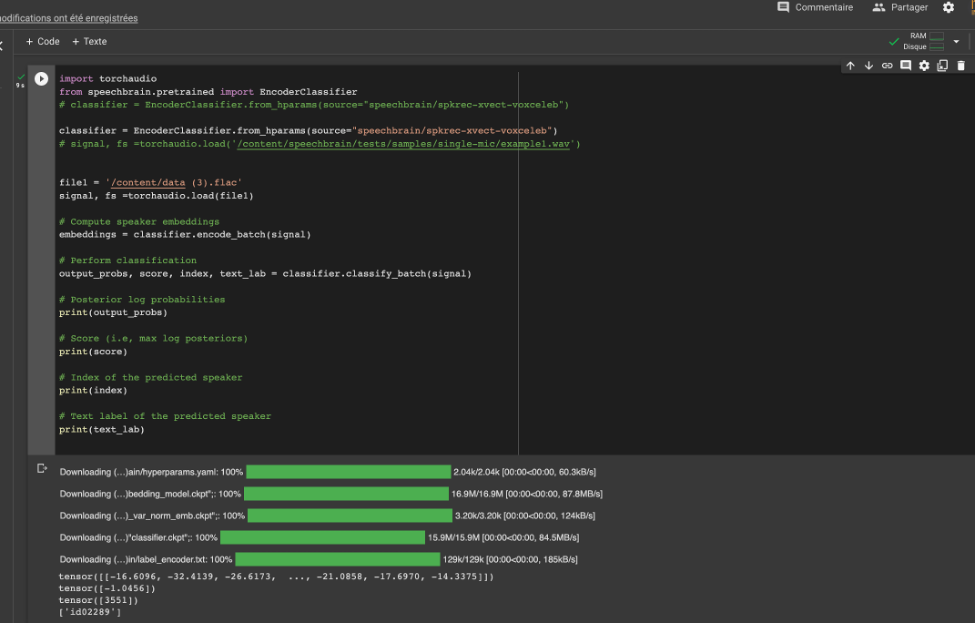
\includegraphics[width=1\textwidth]{3chap27}
	\caption{Préparation du model  }
	\label{fig:3chap27}
\end{figure}

Mais comment cela fonctionne-t-il avec notre model que nous avons formé auparavant ?

\begin{figure}[h]
	\centering
	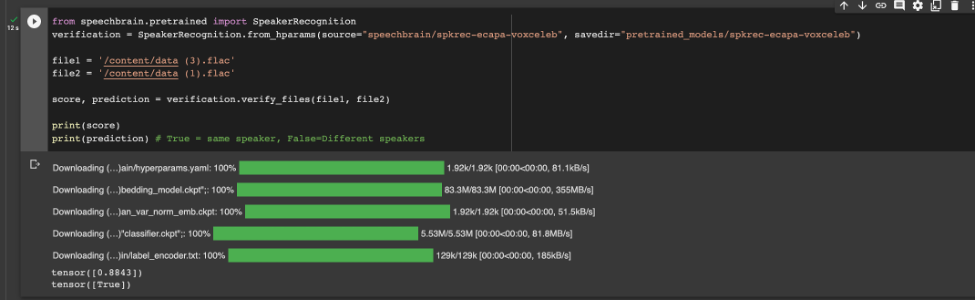
\includegraphics[width=1\textwidth]{3chap28}
	\caption{Inférence sur le modèle pour l'authentification }
	\label{fig:3chap28}
\end{figure}

Exemple d’inférence pour l’authentication. le résultat est contenue dans la variable prédiction (voir figure \ref{fig:3chap28})(True = le locuteur est bien celui dont il s’agit, False=Le locuteur n’est pas celui qu’il prétend). 


\begin{figure}[h]
	\centering
	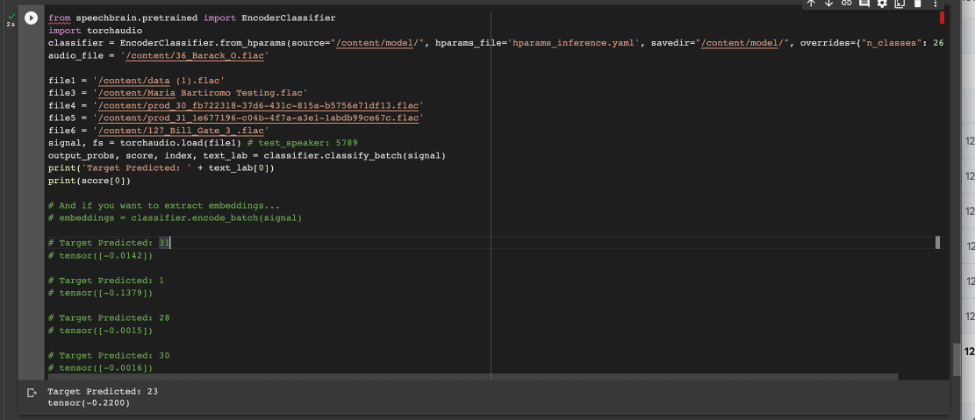
\includegraphics[width=1\textwidth]{3chap29}
	\caption{Inférence sur le modèle pour l'identification }
	\label{fig:3chap29}
\end{figure}
Ici nous avons effectué l’inférence pour l’identification de locuteur ce qui nous a retourné le locuteur avec l’ID 23 (voir figure \ref{fig:3chap29}).

\section{Le développement des Apis}
A cette étape, nous pouvons exporter notre model vers Cloud Storage afin de pouvoir l’utiliser sur notre backend Django.
Le code se presnte comme suit :



\begin{itemize}
    \item UpdateModel cette classe permet de recupere le dernier modeldepui Cloud Storage pour l’utilisation a des fin de reconnaissance. \\\textbf{Requête : GET} \\\textbf{Route : https://api.dev.minfo.com/api/speaker/updatemodel }
	\lstinputlisting[language=Python,  firstline=155, lastline=186]{views.py}

	
    \item \textbf{IdentifySpeaker}: Cette classe permet d’identifier le locuteur. \\\textbf{Requête : POST} \\\textbf{Route : https://api.dev.minfo.com/api/speaker/id}
	\lstinputlisting[language=Python,  firstline=72, lastline=151]{views.py}

    \item \textbf{MatchVoices}: Elle permet d’authentifier un locuteur. \\\textbf{Requête : POST} \\\textbf{Route : https://api.dev.minfo.com/api/speaker/match}
	\lstinputlisting[language=Python,  firstline=12, lastline=46]{views.py}

\end{itemize}

% \begin{lstlisting}[language=Python, caption=Python example]
% 	import numpy as np
		
% 	def incmatrix(genl1,genl2):
% 		m = len(genl1)
% 		n = len(genl2)
% 		M = None #to become the incidence matrix
% 		VT = np.zeros((n*m,1), int)  #dummy variable
		
% 		#compute the bitwise xor matrix
% 		M1 = bitxormatrix(genl1)
% 		M2 = np.triu(bitxormatrix(genl2),1) 
	
% 		for i in range(m-1):
% 			for j in range(i+1, m):
% 				[r,c] = np.where(M2 == M1[i,j])
% 				for k in range(len(r)):
% 					VT[(i)*n + r[k]] = 1;
% 					VT[(i)*n + c[k]] = 1;
% 					VT[(j)*n + r[k]] = 1;
% 					VT[(j)*n + c[k]] = 1;
					
% 					if M is None:
% 						M = np.copy(VT)
% 					else:
% 						M = np.concatenate((M, VT), 1)
					
% 					VT = np.zeros((n*m,1), int)
		
% 		return M
% 	\end{lstlisting}

\addcontentsline{toc}{section}{Conclusion}
\section*{Conclusion}
Dans cette partie, nous avons montré comment créer un model TDNN pour l’authentication et l’identification des locuteurs. Le système proposé contient tous les ingrédients de base pour développer un système de pointe (c'est-à-dire, l'augmentation de données, l'extraction de caractéristiques, l'encodage, la mise en pool statistique, le classificateur, etc.).
Dans le prochain chapitre nous présenterons les résultats obtenus après notre implémentation. 
